\newpage
\section{Continuità}
\begin{definition}[Funzione continua]
    Dato un insieme A ed una funzione $f(x)$ tale che $A \subset \mathbb{R}$, $f: A \longrightarrow \mathbb{R}$, la funzione $f$ si dice \textbf{continua} in $x_0$ se $\forall \: \: \epsilon > 0 \: \: \exists \: \: \delta > 0$ tale che se data una $x \in A$:
    \begin{equation}\label{funzione-continua}
        |x - x_0| < \delta \Longrightarrow |f(x) - f(x_0)| < \epsilon
    \end{equation}
\end{definition}
La condizione scritta sopra [\ref{funzione-continua}] può essere scritta anche tramite due condizioni:
\begin{itemize}
    \item $|x - x_0| < \delta \Longleftrightarrow x_0 - \delta < x < x_0 + \delta$
    \item $|f(x) - f(x_0)| < \epsilon \Longleftrightarrow f(x_0) - \epsilon < f(x) < f(x_0) + \epsilon$
\end{itemize}
\begin{example}
Ora per capire meglio facciamo un esempio di funzione non continua:
\end{example}
Innanzitutto stabiliamo una $f(x)$ e verifichiamo che $f(x)$ in $x_0 = 0$ non è continua.\\ 
\begin{wrapfigure}{r}{8cm}
\vspace{-20pt}
    \centering
    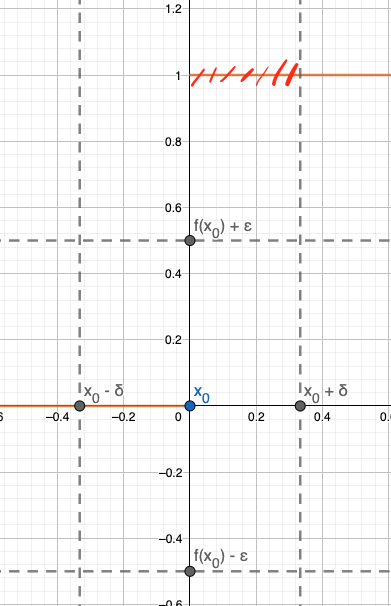
\includegraphics[width=4.8cm, height=5cm]{images/esempio-non-continuita.png}
    \caption{funzione non continua}
    \label{fig:funzione-non-continua}
\end{wrapfigure}

$
  f(x)=\begin{cases}
    0 \: \: se & x \leq 0\\
    1 \: \: se & x > 0
  \end{cases}
$\\ \\ \\
Come prima cosa stabiliamo un $\epsilon = \frac{1}{2}$. Ora, qualunque sia $\delta > 0$ se andiamo a prendere una $x$ tale che $x \in (0, \delta) \Longrightarrow f(x) = 1$ quindi la disuguaglianza $f(x_0) - \epsilon > f(x) < f(x_0) + \epsilon$, che diventerebbe $0 - \frac{1}{2} < f(x) < 0 + \frac{1}{2}$, è falsa. \\ \\
Deduciamo quindi che in $x_0 = 0$ questa funzione non è continua. \\ \\

\begin{definition}
    Dato un insieme A ed una funzione $f(x)$ tale che $A \subset \mathbb{R}$, $f: A \longrightarrow \mathbb{R}$ ed un insieme $B \subset \mathbb{R}$ si dice che $f$ è continua in B e $f$ è continua in ogni punto $x_0 \in B$.
\end{definition}
Se invece si dice semplicemente che $f$ è continua senza specificare il sotto insieme B vuol dire che $f$ è continua in tutti i punti del suo dominio A.
\begin{example}
    Esempio basato sulla funzione vista sopra:\\\\
    $
      f(x)=\begin{cases}
        0 \: \: se & x \leq 0\\
        1 \: \: se & x > 0
      \end{cases}
    $ \hspace{1cm}
    $f$ è continua in $(-\infty, 0) \cup (0, +\infty)$ 
\end{example}

\subsection{Permanenza del segno}
\begin{theorem}[Permanenza del segno]\label{permanenza-segno}
    Dato un insieme A ed una funzione $f$ tale che $A \subset \mathbb{R}$, $f: A \longrightarrow \mathbb{R}$, $x_0 \in A$. Se $f$ è continua in $x_0$ e $f(x_0) > 0$ allora $\exists \: \: \delta > 0$ t.c. se $x \in A$ è $|x - x_0| < \delta \longrightarrow f(x) > 0$. Analogo risultato se $f(x_0) < 0$.
    \begin{demostration}
    Sappiamo che $f(x_0) > 0$. Ora scegliamo un $\epsilon = \frac{f(x_0)}{2}$ ed utilizziamolo nella definizione di continuità:
    \begin{equation}
        \exists \: \: \delta > 0 \: \: | \: \: x \in A, |x - x_0| < \delta \Longleftarrow |f(x) - f(x_0)| < \epsilon
    \end{equation}
    Ciò che risulta dalle condizioni poste dalla continuità è che:
    \begin{equation}
        f(x_0) - \epsilon < f(x) < f(x_0) + \epsilon
    \end{equation}
    Se prendiamo la prima parte $f(x_0) - \epsilon < f(x)$ e facciamo le dovute sostituzioni risulta che:
    \begin{equation}
        f(x_0) - \frac{f(x_0)}{2} < f(x)
    \end{equation}
    Visto che $f(x_0) - \frac{f(x_0)}{2}$ è sempre maggiore di 0 risulta anche che $f(x)$ è maggiore di 0. $\blacksquare$
    \end{demostration}
    \begin{corollaries}\label{collorartio-permanenza-segno}
        Se $f$ è continua in $x_0$ $f: A \longrightarrow \mathbb{R}$, $x_0 \in A$ e $f(x_0) > M$ con $M \in \mathbb{R}$, $x \in A$, $|x - x_0| < \delta \Longrightarrow f(x) > M$. (Vale anche con $f(x_0) < M \Longrightarrow f(x) < M$)
    \end{corollaries}
    \begin{demostration}[Dimostrazione del corollario \ref{collorartio-permanenza-segno}]
        La dimostrazione di questo corollario è immediata e si fa applicando al teorema precedente \ref{permanenza-segno} la funzione $g(x) = f(x) - M$, perché se la funzione $f(x) - M > 0$ è come dire $f(x) > M$. $\blacksquare$
    \end{demostration}
\end{theorem}

\subsection{Continuità con operazioni fra funzioni}
\begin{theorem}
    Prendendo due funzioni $f$ e $g$ continue in un punto $x_0$ allora le funzioni $f + g$, $f * g$ e $|f|$, se inoltre $f(x_0) \neq 0$ allora anche $\frac{1}{f}$ è continua.
    \begin{corollaries}
        Prendendo due funzioni $f$ e $g$ continue in un punto $x_0$ allora $\frac{f}{g}$ è continua se $g(x_0) \neq 0$
    \end{corollaries}
\end{theorem}

\subsection{Funzioni invertibili e continuità}
\begin{proposition}\label{proposizione-funzione-inversa}
    Prendendo due insiemi I (I deve essere un intervallo) e B tale che $I \subset \mathbb{R}$ e $B \subset \mathbb{R}$ ed una funzione $f: I \longrightarrow B$, se $f$ è continua in $I$ ed è invertibile allora $f^{-1}$ è continua in B.
\end{proposition}
\begin{observation}
    Possiamo osservare che ipotesi della proposizione \ref{proposizione-funzione-inversa} dice che il domino sia un intervallo, questo non può essere omesso. 
\end{observation}
\begin{example}
    Verifichiamo questa osservazione con un' esempio:\\
    Prendiamo una funzione $f(x)$ definita in $f: (-\infty, 1] \cup (2, +\infty) \longrightarrow \mathbb{R}$ \: \: \: $f(x) = 
    \begin{cases}
        x \: \: se & x \leq 1 \\
        x - 1 \: \: se & x > 1
    \end{cases}
    $\\
    Qui di seguito le rappresentazioni della funzione $f(x)$ e della sua inversa $f(x)^{-1}$
\end{example}
\begin{figure}[h!]
    \vspace{10pt}
    \begin{subfigure}{.5\textwidth}
        \centering
        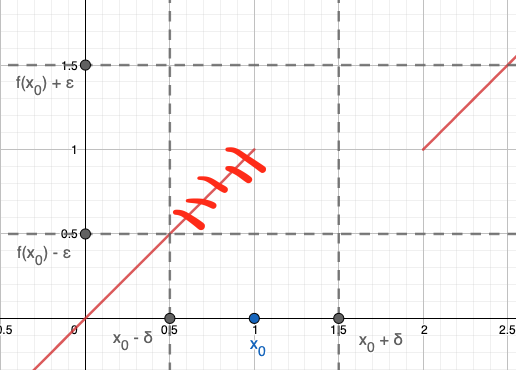
\includegraphics[width=5.5cm]{images/esempio1-osservazione-prop1.png}
        \caption{Osservazione proposizione \ref{proposizione-funzione-inversa}, funzione $f(x)$}
        \label{fig:es1-prop1}
    \end{subfigure}
    \begin{subfigure}{.5\textwidth}
        \centering
        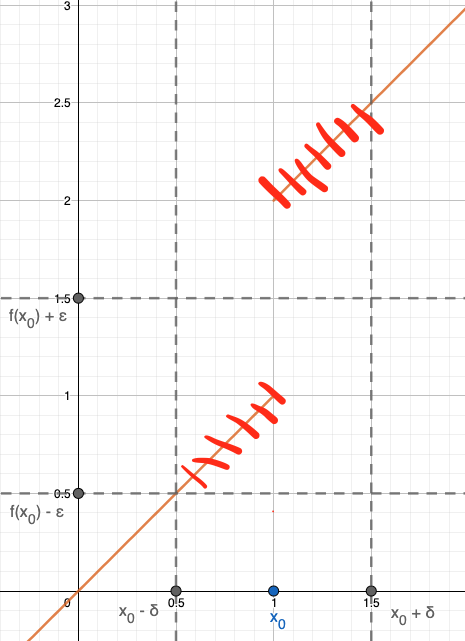
\includegraphics[width=4.2cm, height=5.2cm]{images/esempio2-osservzione-prop1.png}
        \caption{Osservazione proposizione \ref{proposizione-funzione-inversa}, funzione $f(x)^{-1}$}
        \label{fig:es2-prop1}
    \end{subfigure}
\end{figure}
\begin{itemize}
    \item \textbf{Domanda 1°:} $f$ è continua in $x_0 = 1$?\\
    La risposta a questa prima domanda è SI, essendo che noi andiamo a considerare solo i punti all'interno del dominio, quindi la parte compresa fra 1 e 2, dove la funzione presenta una discontinuità, non si considera.
    \item \textbf{Domanda 2°:} $f$ è continua in $x_0 = 2$?\\
La risposta in questo caso è che non ha senso considerare il punto $x_0 = 2$ visto che 2 non fa parte del dominio.
\end{itemize}
Quindi $f$ è continua in tutto il suo dominio. Essendo $f$ continua in tutto il suo dominio allora teoricamente $f^{-1}$ è una funzione invertibile. \\ \\
Possiamo però vedere che la funzione $f^{-1}$, figura [\ref{fig:es2-prop1}] non è continua in $x_0 = 1$ perché essendo la funzione inversa $f^{-1}$ è definita come $f^{-1}: \mathbb{R} \longrightarrow (-\infty, 1] \cup (2, +\infty)$, quindi dobbiamo considerare come dominio tutto $\mathbb{R}$, così facendo ci sono dei punti, in particolare con $x > 0$ che non rientrano nell'intervallo fra $f(x_0) - \epsilon$ e $f(x_0) + \epsilon$ . \\ \\
In conclusione da questo esempio deduciamo che, se $f$ non è definita in un intervallo potrebbe succedere che $f^{-1}$ non è continua anche se $f$ è continua.

\subsection{Continuità delle funzioni elementari}
$f(x) = x$ è una funzione continua. Da questa considerazione segue che tutte le funzioni con polinomi sono continue.
\begin{note}
    Ricorda che anche le funzioni costanti sono sempre continue
\end{note}
Definiamo in maniera generica così una funzione formata da polinomi continua:
\begin{equation}
    P(x) = a_n * x^n + a_{n-1} * x^{n-1} + .... + a_1 * x + a_0 \: \: con \: \: a_0, a_1, ..., a_n \in \mathbb{R}
\end{equation}
Quindi: $x^2 = x * x$ è continua \hspace{.5cm} $x^3 = x^2 * x$ è continua \hspace{.5cm} $x^n$ è continua $\: \: \forall x \in \mathbb{N}$ \\ \\
Le funzioni razionali sono continue nel loro insieme di definizione. Le funzioni razionali sono uguali a quoziente di polinomi:
$f(x) = \frac{p(x)}{q(x)}$ con $p,q$ polinomi, la funzione $f(x)$ è definita se $q(x) \neq 0$.\\ \\
Assumendo che $e^x$, $\sin{x}$, $\cos{x}$ sono funzioni continue quindi anche $\log{x}$, $\arcsin{x}$, $\arccos{x}$, $\tan{x}$, $\arctan{x}$ sono continue.

\subsection{Continuità fra composizione di funzioni}
\begin{theorem}
    Date due funzioni $f: A \longrightarrow \mathbb{R}$ e $g: B \longrightarrow \mathbb{R}$, ed un $x_0 \in A$, $y_0 = f(x_0) \in B$.
    Se $f$ è continua in $x_0$ e $g$ è continua in $y_0$ allora $g \bullet f$ è continua in $x_0$.
\end{theorem}
\begin{example}
    Facciamo un esempio usando la funzione $e^{\cos{x}}$.\\
    $e^{\cos{x}}$ è una funzione continua perché è la composizione di $f(x) = \cos{x}$, funzione continua, e $g(x) = e^y$, pure essa funzione continua.
\end{example}
\begin{observation}
    Data una $f: [a, b] \longrightarrow \mathbb{R}$ continua in $[a, b]$ allora sup($f(x)$) con $x \in (a, b)$ = sup($f(x)$) con $x \in [a, b]$. E ugualmente inf($f(x)$) con $x \in (a, b)$ = inf($f(x)$) con $x \in [a, b]$.
\end{observation}
\begin{example}
    $f(x) = x^2$ con $f: [0,1] \longrightarrow \mathbb{R}$\\
    sup($f(x)$) = $f(1) = 1$ con $x \in [0, 1]$ \hspace{.5cm} sup($f(x)$) = $f(1) = 1$ con $x \in (0, 1)$ \footnote{Ricorda che sup(imm($f(x)$)) = sup(0, 1) = 1}
\end{example}

\subsection{Teorema degli zeri}
\begin{theorem}[Teorema degli zeri]
    Data una $f: [a, b] \longrightarrow \mathbb{R}$ continua. Se $f(a) \cdot f(b) < 0$ allora $\exists c \in (a, b)$ tale che $f(c) = 0$
\end{theorem}
Questo teorema dice che prendendo una funzione, che deve essere obbligatoriamente continua, se i valori di $f(x)$ nei due estremi moltiplicati fra di loro risultano minori di 0 la funzione passa per 0 in un ponto $c$ e questo accade perché se il prodotto fra i due estremi torni inferiore a 0 vuol dire che hanno segno discorde.\\
\begin{example}
    Facciamo un esempio di un caso in cui la funzione NON è continua:
\end{example}
\begin{wrapfigure}{r}{5cm}
    \vspace{-10pt}
    \centering
    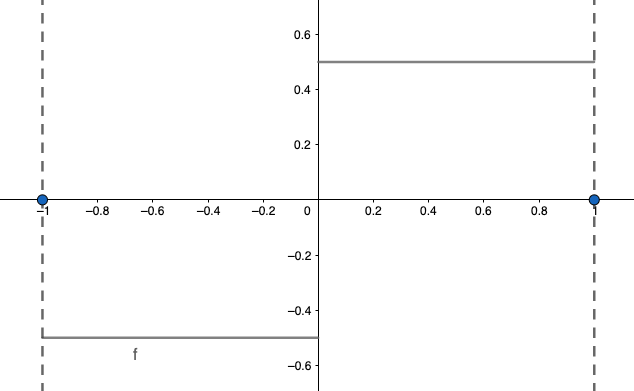
\includegraphics[width=4.5cm, height=2cm]{images/esempio-teorema-zeri.png}
    \caption{$f(x) = [x] + \frac{1}{2}$}
    \label{fig:esempio-teorema-zeri}
\end{wrapfigure}
Prendiamo $f(x) = [x] + \frac{1}{2}$ \: $f: [1, -1] \longrightarrow \mathbb{R}$\\ \\
Se ora prendiamo la f(x) nei due estremi e facciamo il prodotto torna che: \\
$f(1) \cdot f(-1) < 0$ ma $\nexists x \in [-1.1]$ t.c. $f(x) = 0$ come possiamo vedere nell'immagine \ref{fig:esempio-teorema-zeri}.\\ \\

\subsection{Teorema valori intermeti}
\begin{theorem}[Teorema dei valori intermedi]
    Prendendo un intervallo $I \subset R$, ed una funzione $f: I \longrightarrow \mathbb{R}$ continua, allora $f(I)$ è un intervallo.
\end{theorem}
Questo teorema dice che se il nostro dominio è un intervallo e la $f$ è continua all'ora anche il codominio o immagine di $f$ sarà un intervallo.
\begin{corollaries}
    Prendendo sempre un $I \subset R$, una funzione $f: I \longrightarrow \mathbb{R}$ continua, se $f$ assume $y_1$ e $y_2$ allora assume anche tutti i valori compresi fra $y_1$ e $y_2$.
\end{corollaries}

\subsection{Teorema di Weirstrass}
\begin{theorem}[Teorema di Weirstrass]
    Data una funzione $f: [a, b] \longrightarrow \mathbb{R}$ continua. Allora f ha massimo e minimo.
\end{theorem}
\begin{note}
    Notare che $a,b \in \mathbb{R}$ e non in $\overline{\mathbb{R}}$ perché $a, b \neq \pm \infty$ e gli estremi devono essere compresi.
\end{note}
\begin{example}
    Facciamo ora un esempio per confermare come il teorema di Weirstrass possa valore solo con un intervallo chiuso:\\
    Dato $f(x) = \frac{1}{x}$ con $f(x): (0, 1] \longrightarrow \mathbb{R}$ \\ \\in questo caso $f$ ha come dominio un intervallo non chiuso a sinistra\\
    $f$ è continua ma non ha max perché sup($f$) = $+\infty$
\end{example}
\begin{example}
    Facciamo ora un esempio per confermare come il teorema di Weirstrass possa valore solo con un intervallo limitato:\\
    Dato $f(x) = \arctan{x}$ con $f(x): \mathbb{R} \longrightarrow \mathbb{R}$ \\ \\in questo caso $f$ è una funzione continua definita come $-\frac{\pi}{1} < f(x) < \frac{\pi}{2}$\\
    Possiamo notare però che f non toccherà mai ne $-\frac{\pi}{2}$ ne $\frac{\pi}{2}$ e quindi non ha ne massimo ne minimo.
\end{example}